\chapter{Methodology}
This chapter summarizes the methodology used to develop the recovery system for this thesis.
In short, the recovery system is developed example-driven using the model of a fictional Human Resource Management System used by the 101wiki\footnote{\url{https://101wiki.softlang.org/} (retrieved \formatdate{12}{11}{2017})} for its contributions.

\section{The 101HRMS Model}
The 101 Human Resource Management System\footnote{\url{https://101wiki.softlang.org/101:@system} (retrieved \formatdate{12}{11}{2017})} (101HRMS) provides a simple model of a company with many departments and employees.
Figure \ref{figure:101HRMSModel} shows an UML class diagram of a variant of the model where each entity also has an ID attribute.

\begin{figure}[h!]
\begin{center}
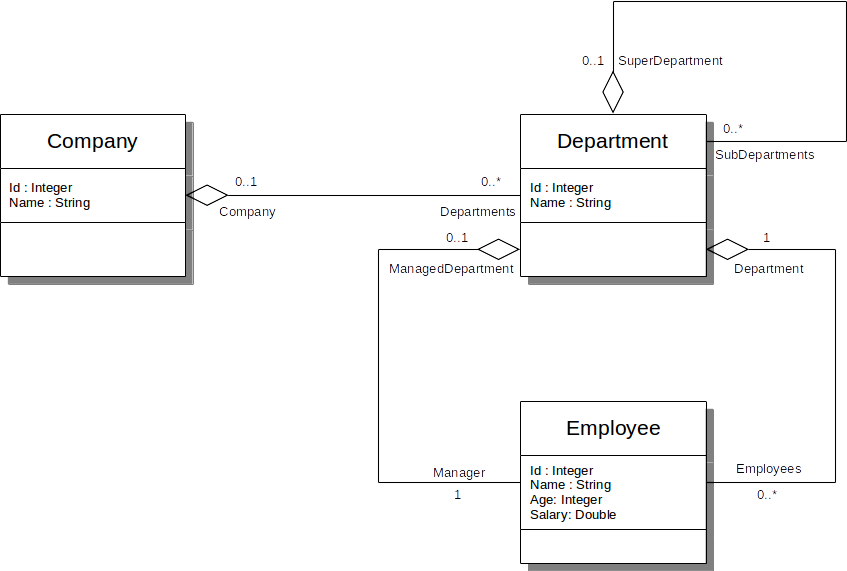
\includegraphics[scale=.5]{images/101HRMSModel.png}
\end{center}
{
\scriptsize 
This UML class diagram depicts the model of the 101 Human Resource Management System.
It consists of simple companies with nested departments and employees mapped to the latter.
}
\caption{The 101 Human Resource Management System Model}
\label{figure:101HRMSModel}
\end{figure}

The 101HRMS model consists of companies attributed with a name.
Each company accumulates departments.
Each department is also attributed with a name, aggregates employees and has one employee acting as manager.
Departments can further be refined into sub-departments.
Each employee is attributed with a name, an age and a salary.

\section{The 101HRMS Example Corpus}
The actual 

\begin{figure}[h!]
\begin{center}
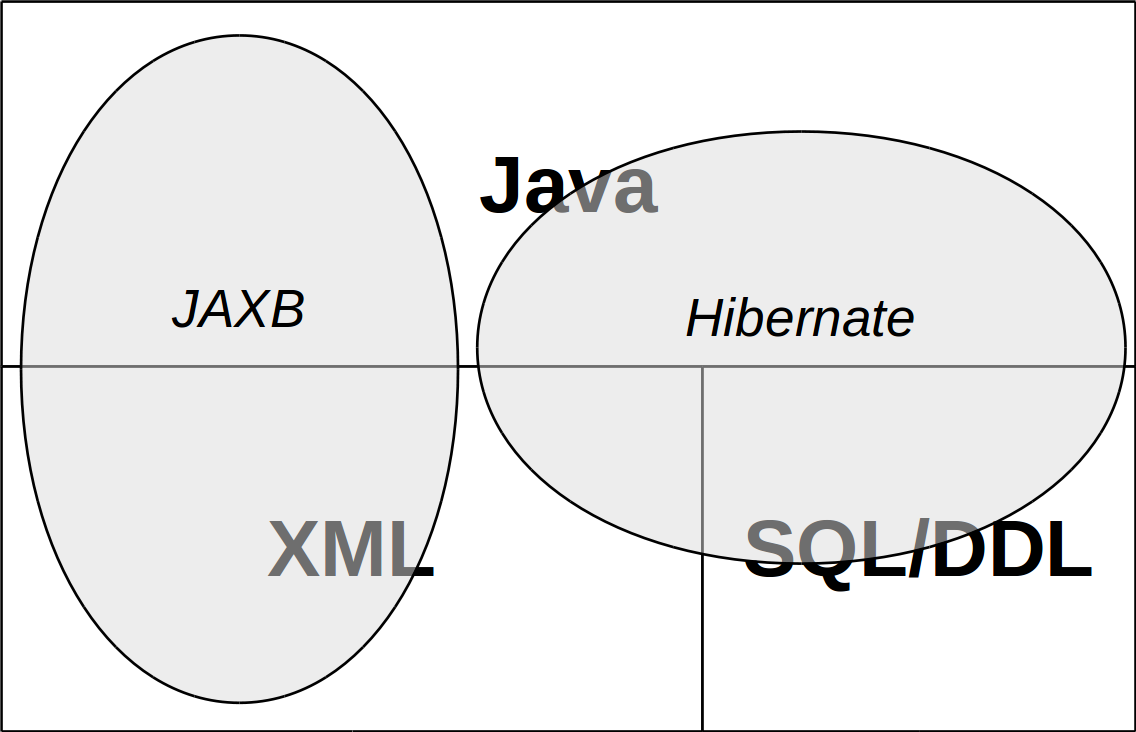
\includegraphics[scale=.5]{images/JORXDomains.png}
\end{center}
{
\scriptsize 
This UML class diagram depicts the model of the 101 Human Resource Management System.
It consists of simple companies with nested departments and employees mapped to the latter.
}
\caption{Example Java O/R/X Domains}
\label{figure:ExampleJORXDomains}
\end{figure}

%\section{Link Proper Part Ratio}
%The ratio between all proper parts of two artifacts and the proper parts of the same artifacts in a relationship.
%
%\begin{align*}
%\pi_{R,A_1,A_2} = \frac{|\{ (p_1,p_2) \in R : p_1 \properPartOf A_1 \wedge p_2 \properPartOf A_2 \}|}{|\{ p : p \properPartOf A_1 \vee p \properPartOf A_2\}|}
%\end{align*}